It is also important to choose a correct optimizer in order for a model to converge as fast as possible. Here, three different optimizers have been tried out --- namely, SGD, Adam and Adadelta. One can evaluate the quiality of an optimization technique based on the speed of convergence and a value towards which the training has converged. As can be seen in Figure \ref{fig:optimizers} the SGD optimizer performed the worst, while Adam and Adadelta optimizer performed similarly with Adadelta converging to slightly better values in the end. SGD optimizer converges both slower and towards a higher loss, whereas SGD converges slightly slower than Adam, however to a lower loss. One can see in Figure \ref{fig:optimizers} that Adam optimizer has required some fine-tuning of the learning rate from 0.001 to 0.0001 to achieve the best result. Both Adadelta and Adam can be used for model optimization in this dataset, however adadelta optimizer was chosen as it has converged to a lower values of loss. The experiments were conducted on the truncated dataset of nuclei images using PCC loss.

\begin{figure}[H]
	\begin{center}
		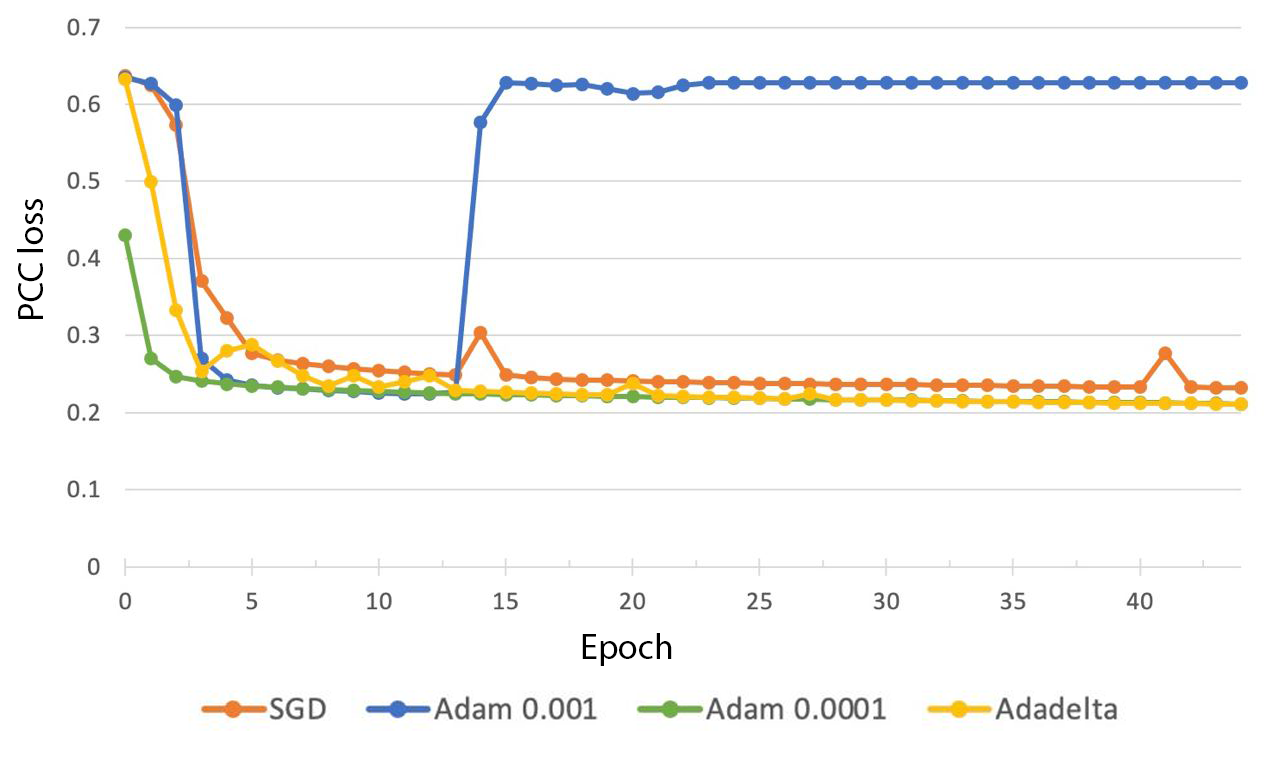
\includegraphics[width=0.8\linewidth]{bilder/model training/optimizer-comparison.png}
		\caption{Comparison of convergence for different optimizers}\label{fig:optimizers}
	\end{center}
\end{figure}
